\documentclass[12pt]{article}

\usepackage{tikz}
  \usetikzlibrary{arrows,calc,shapes}
\usepackage{xspace}

\newcommand{\CASL}{\textrm{\textsc{Casl}}\xspace}
\newcommand{\CC}{\textrm{\textsc{Csp}-\textsc{Casl}}\xspace}

\begin{document}

\section{Introduction}

This is a specification of an online shopping system.  There are 4
components to the system: the customer, the warehouse, the payment
system and the coordinator. These components are connected in a star
shape fashion as below:

\tikzstyle{process}=[draw, rounded corners,minimum height=0.7cm, minimum width=2cm]
\tikzstyle{short}=[node distance=3cm]
\tikzstyle{channel}=[<->, >=triangle 60, shorten <=2pt, shorten >=2pt]
\tikzstyle{link}=[shorten <=5pt, shorten >=5pt]
\tikzstyle{bubble}=[shade, top color=blue!30, bottom color=blue!10,
                      ellipse callout, draw]
\begin{center}
  \begin{tikzpicture}[auto, node distance=3cm]
    \node [process] (Customer){Customer};
    \node [process] (Coordinator) at ($(Customer) + (3.5,0)$) {Coordinator};
    \node [process,short,anchor=south west] (Warehouse) at ($(Coordinator) + (2,1)$) {Warehouse};
    \node [process,short,anchor=north west] (PaymentSystem) at ($(Coordinator) + (2,-1)$) {Payment System};
    \draw [channel] (Customer) -- node(C-C){C\_C} (Coordinator);
    \draw [channel] (Coordinator.north east) -- node{C\_W} (Warehouse.south west);
    \draw [channel] (Coordinator.south east) -- node[swap](C-PS){C\_PS} (PaymentSystem.north west);

    \node [bubble,callout pointer shorten=6pt,callout absolute pointer={(Customer.south)}] at ($(Customer) + (-1,-2)$) {Processes};
    \node [bubble,callout absolute pointer={(C-PS.south west)}] at ($(C-C) + (1,-2)$) {Data};
  \end{tikzpicture}
\end{center}


C\_C (Channel Customer) is the channel between the customer and the
coordinator.

C\_W (Channel Warehouse) is the channel between the coordinator and the
warehouse.

C\_PS (Channel PaymentSystem) is the channel between the coordinator
and the payment system.

\section{Abstraction Levels}

We model the following 3 levels of abstraction:
\begin{description}
\item [Architectural Level (Arch):] Here the structure of the system is
   specified. Basically this is just the picture above.
\item [Abstract Component Level (ACL):] Here the types and order of the
   messages are specified.
\item [Concrete Component Level (CCL):] Here the actual messages are specified
   up to representation.
\end{description}

\section{The Structure of Each Abstraction Level}

Each of the abstraction levels has the following structure:

\begin{center}
  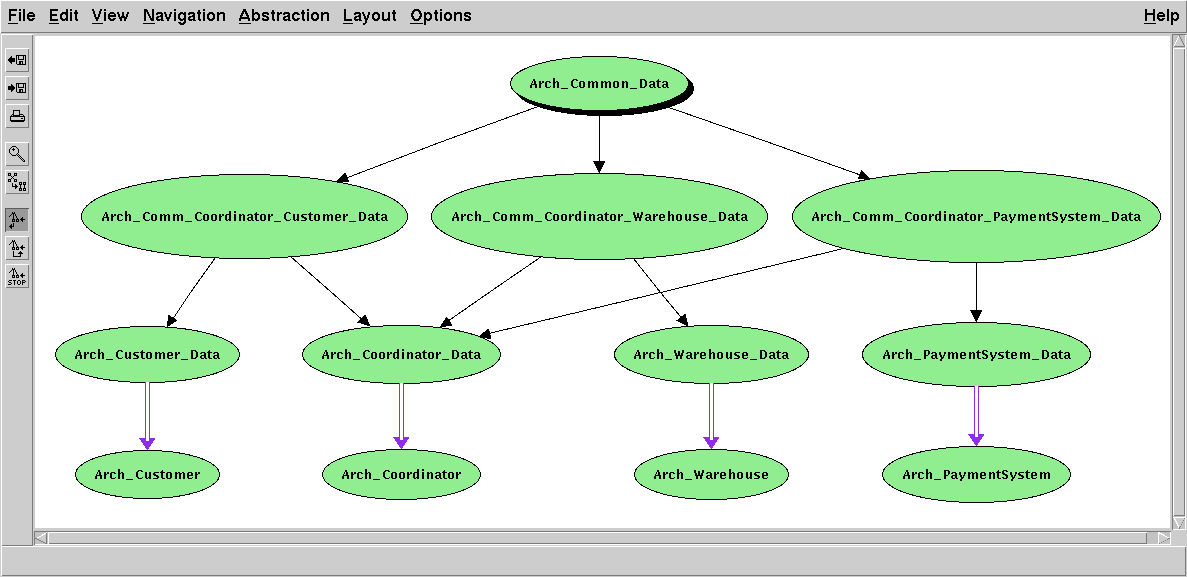
\includegraphics[width=0.9\textwidth]{Hets.png}
\end{center}

The first row contains a single \CASL specification of the common data
for all channels. The second row contains \CASL specifications of
data for each channel. The third row contains \CASL specifications
for each component's data. The forth row contains \CC specifications
for each component.

\section{Goals of the Online Shopping System}

Customers should be able to:
\begin{itemize}
    \item Get a catalogue of items,
    \item View Items in their basket,
    \item Add items to their basket,
    \item Remove items from their basket,
    \item Cancel their order then quit and
    \item Checkout their basket.
\end{itemize}
The customer makes the choice of which actions they want to perform.

The coordinator should offer the customer the ability to:
\begin{itemize}
    \item Get a catalogue of items,
    \item View Items in their basket,
    \item Add items to their basket,
    \item Remove items from their basket,
    \item Cancel their order then quit and
    \item Checkout their basket.
\end{itemize}

The coordinator allows all the possible actions and chooses the same
action as the customer based on the customers requests.

We force the customer to make a login request, after which the
coordinator decides which course of action should be taken: either a
good login behaviour followed by allowing the customer into the shop
or a bad login behaviour which returns the customer to the login
phase.

When the customer issues a view catalogue request, then the coordinator
should send the catalogue back to the customer in a view catalogue
response. The catalogue is a store in the coordinator and contains all
products, even products that the warehouse has not got in stock.

When the customer issues a view basket request, then the coordinator
should send the basket back to the customer.

When the coordinator receives an add item request from the customer,
the coordinator should try to reserve that item in the warehouse. If
the reservation is successful then the item is added to the basket and
the customer is informed that the request was successful using an add
item response. If the item was not reserved then the customer is
informed that the request failed using an add item response.

When the coordinator receives a remove item request from the customer,
the coordinator should check if the item is in the basket and if so
release that item in the warehouse and report success. If the item was
not in the basket then the customer should be informed of this.

The warehouse offers the coordinator at any time to release a reserved
item. If an item release request is made for an item that is not
reserved then the warehouse makes no guarantees what happens.

When the coordinator receives a checkout command, the coordinator
should calculate the invoice from the basket and catalogue and send
this invoice to the customer. The customer at this point can cancel
the checkout and return to the state before the checkout request was
issued. Otherwise the customer can send a checkout confirm message to
the coordinator which includes all necessary payment data and delivery
data. The coordinator then asks the Payment System to take payment
using the customers payment details and invoice that was produced
earlier in this dialogue. The Payment System reports to the
coordinator the status of the payment. If the Payment System fails to
take payment then the customer is notified of a failed checkout
request and the customer returns to the state before the checkout
request was issued. Otherwise if the payment was successful then the
coordinator tells the warehouse to deliver the reserved items to the
delivery address (this process cannot fail). The customer is then
informed of a successful checkout. The basket is then empty.

The Basket is a data structure stored in the coordinator. The basket
should mirror at all times (but not during a dialogue) the reserved
items in the warehouse. The warehouse is assumed to have no reserved
items at the start. The basket in the coordinator is assumed to be
empty at the start.

\end{document}
